\documentclass[tikz,border=6pt]{standalone}
\usetikzlibrary{positioning,arrows.meta,shapes.multipart}

\begin{document}
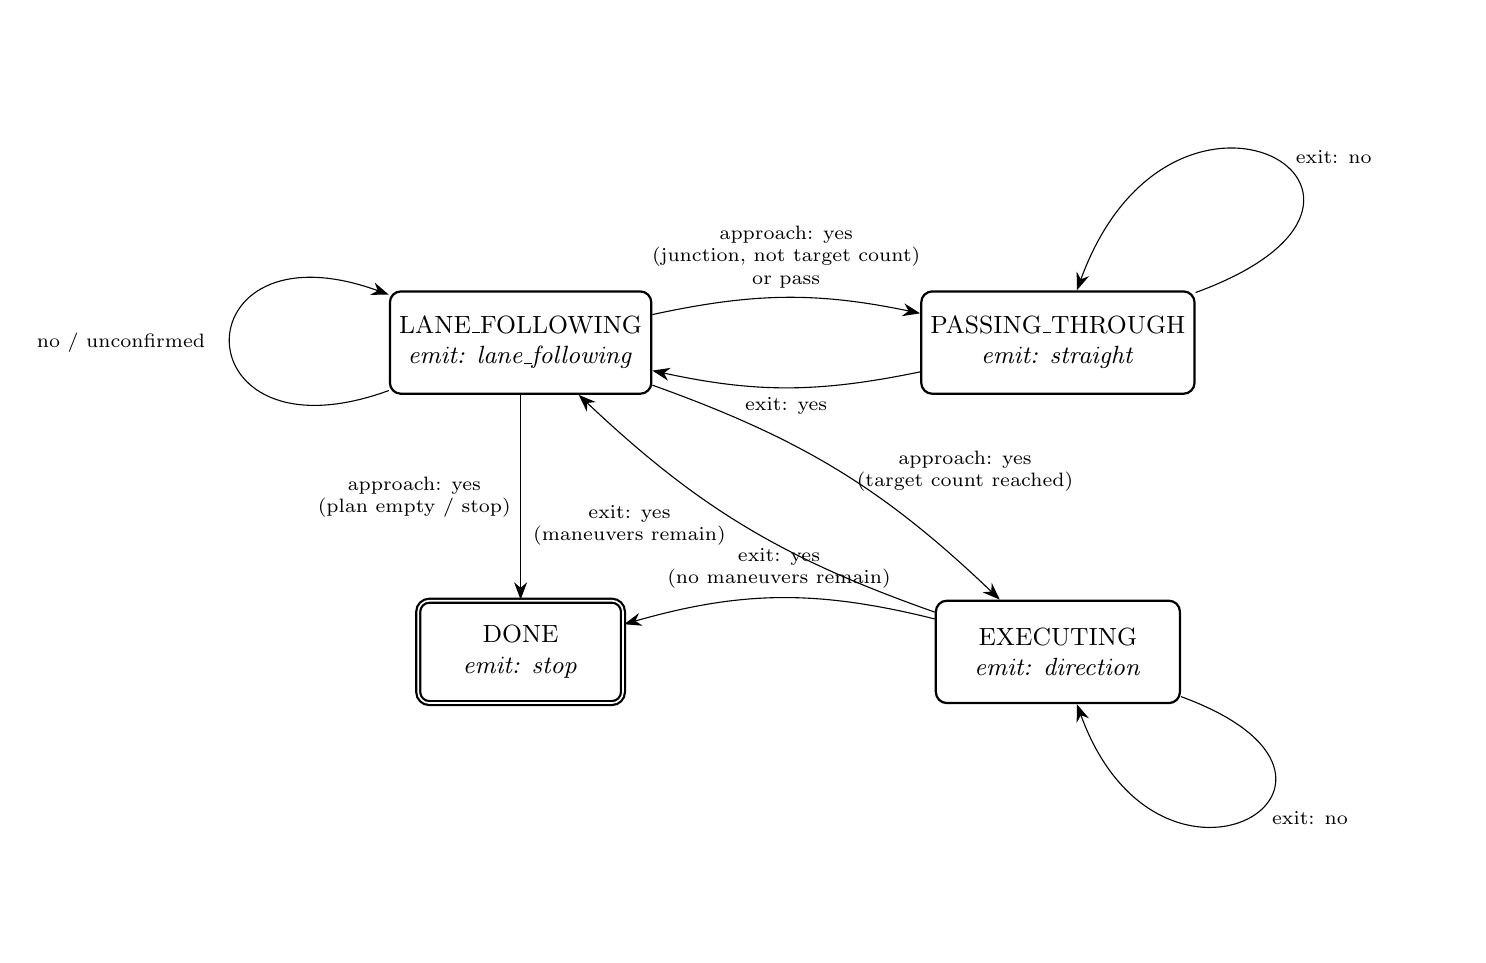
\begin{tikzpicture}[
  >={Stealth[length=2.2mm]},
  state/.style={rectangle, rounded corners, draw=black, thick, minimum width=3.1cm, minimum height=1.3cm, align=center, font=\small},
  donestate/.style={state, double, minimum width=2.6cm},
  lbl/.style={font=\scriptsize, align=center, midway},
  node distance=2.6cm and 3.4cm
]

\node[state] (lf) {LANE\_FOLLOWING\\\textit{emit: lane\_following}};
\node[state, right=of lf] (pt) {PASSING\_THROUGH\\\textit{emit: straight}};
\node[state, below=of pt] (ex) {EXECUTING\\\textit{emit: direction}};
\node[donestate, below=of lf] (done) {DONE\\\textit{emit: stop}};

% LANE_FOLLOWING transitions
\draw[->] (lf) to[bend left=12] node[lbl, above] {approach: yes\\(junction, not target count)\\or pass} (pt);
\draw[->] (lf) to[bend left=12] node[lbl, right, xshift=1mm] {approach: yes\\(target count reached)} (ex);
\draw[->] (lf) -- node[lbl, left] {approach: yes\\(plan empty / stop)} (done);
\draw[->] (lf) to[out=200,in=160,looseness=6] node[lbl, left, xshift=-2mm] {no / unconfirmed} (lf);

% PASSING_THROUGH transitions
\draw[->] (pt) to[bend left=12] node[lbl, below] {exit: yes} (lf);
\draw[->] (pt) to[out=20,in=70,looseness=6] node[lbl, right, xshift=2mm] {exit: no} (pt);

% EXECUTING transitions
\draw[->] (ex) to[bend left=12] node[lbl, left, xshift=-1mm] {exit: yes\\(maneuvers remain)} (lf);
\draw[->] (ex) to[bend right=15] node[lbl, above] {exit: yes\\(no maneuvers remain)} (done);
\draw[->] (ex) to[out=-20,in=-70,looseness=6] node[lbl, right, xshift=2mm] {exit: no} (ex);

\end{tikzpicture}
\end{document}
